\documentclass{article}\usepackage[]{graphicx}\usepackage[]{color}
% maxwidth is the original width if it is less than linewidth
% otherwise use linewidth (to make sure the graphics do not exceed the margin)
\makeatletter
\def\maxwidth{ %
  \ifdim\Gin@nat@width>\linewidth
    \linewidth
  \else
    \Gin@nat@width
  \fi
}
\makeatother

\definecolor{fgcolor}{rgb}{0.345, 0.345, 0.345}
\newcommand{\hlnum}[1]{\textcolor[rgb]{0.686,0.059,0.569}{#1}}%
\newcommand{\hlstr}[1]{\textcolor[rgb]{0.192,0.494,0.8}{#1}}%
\newcommand{\hlcom}[1]{\textcolor[rgb]{0.678,0.584,0.686}{\textit{#1}}}%
\newcommand{\hlopt}[1]{\textcolor[rgb]{0,0,0}{#1}}%
\newcommand{\hlstd}[1]{\textcolor[rgb]{0.345,0.345,0.345}{#1}}%
\newcommand{\hlkwa}[1]{\textcolor[rgb]{0.161,0.373,0.58}{\textbf{#1}}}%
\newcommand{\hlkwb}[1]{\textcolor[rgb]{0.69,0.353,0.396}{#1}}%
\newcommand{\hlkwc}[1]{\textcolor[rgb]{0.333,0.667,0.333}{#1}}%
\newcommand{\hlkwd}[1]{\textcolor[rgb]{0.737,0.353,0.396}{\textbf{#1}}}%
\let\hlipl\hlkwb

\usepackage{framed}
\makeatletter
\newenvironment{kframe}{%
 \def\at@end@of@kframe{}%
 \ifinner\ifhmode%
  \def\at@end@of@kframe{\end{minipage}}%
  \begin{minipage}{\columnwidth}%
 \fi\fi%
 \def\FrameCommand##1{\hskip\@totalleftmargin \hskip-\fboxsep
 \colorbox{shadecolor}{##1}\hskip-\fboxsep
     % There is no \\@totalrightmargin, so:
     \hskip-\linewidth \hskip-\@totalleftmargin \hskip\columnwidth}%
 \MakeFramed {\advance\hsize-\width
   \@totalleftmargin\z@ \linewidth\hsize
   \@setminipage}}%
 {\par\unskip\endMakeFramed%
 \at@end@of@kframe}
\makeatother

\definecolor{shadecolor}{rgb}{.97, .97, .97}
\definecolor{messagecolor}{rgb}{0, 0, 0}
\definecolor{warningcolor}{rgb}{1, 0, 1}
\definecolor{errorcolor}{rgb}{1, 0, 0}
\newenvironment{knitrout}{}{} % an empty environment to be redefined in TeX

\usepackage{alltt}
\title{Laboratory Assignment 3} 
\author{Katherine Wolf}
\date{\today}

% list of latex packages you'll need
\usepackage{float}  % for tables
\usepackage{mathtools}  % for mathematical symbols
\usepackage{bm}  % to bold mathematical symbols like betas
\usepackage{scrextend}  % to indent subsections
\usepackage{xltxtra}
\usepackage{fontspec}
\usepackage{xunicode}
\usepackage[dvipsnames]{xcolor}
\usepackage{soul}  % get underlines
\usepackage[skip=0.5\baselineskip]{caption}  % control caption printing space
\usepackage{longtable}
\usepackage{amsmath}
\usepackage{amsfonts}

% set fonts
\setmainfont{Georgia}
\setsansfont[Scale=MatchLowercase]{Arial}  % sets the sans font
\setmonofont[Scale=MatchLowercase]{inconsolata}  % sets the monospace font

% make special code formatting
\NewDocumentCommand{\codeword}{v}{%
  \texttt{\textcolor{RoyalPurple}{#1}}%
}

% set the margins of the document
\usepackage[top=1in, bottom=1in, left=.5in, right=.5in]{geometry}
\setlength\parindent{0pt}

% make quick draft versus final versions
\newif\ifdraft  % make draft command
\draftfalse  % one of these must be commented
% \drafttrue  % one of these must be commented

% end the preamble and begin the document
\IfFileExists{upquote.sty}{\usepackage{upquote}}{}
\begin{document}




  \vspace*{-2cm}
  {\let\newpage\relax\maketitle}
  
\maketitle

\ifdraft

\textbf{Read all questions carefully before answering.} You may work in small groups of no more than 3 individuals and turn in a single assignment (and everyone in the group will receive the same grade). Work through the entire assignment individually first, then come together to discuss and collaborate. Please type your responses, \textbf{show your work, and please keep answers brief}.

\section*{Directions}

\vspace{2mm}

Use the dataset \codeword{frmgham_recoded.Rdata} and code provided herein to explore the relationship between smoking status at baseline and time to death in the Framingham cohort.

\fi



\ifdraft

\vspace{2mm}

The relevant variables for this analysis are:
\begin{itemize}
  \item \codeword{time_yrs} (time of entry into study)
  \item \codeword{death} (indicator of death [=1] or censored [=0])
  \item \codeword{cursmoke} (indicator of current smoking status: yes (1) vs. no (0))
  \item \codeword{age} (age in years)
  \item \codeword{sex} (variable denoting male (1) or female (2); \textbf{use 1 as referent category})
  \item \codeword{educ} (educational status, nominal categories 1-4; \textbf{use 1 as referent category})
\end{itemize}

Adapting the code presented in the lecture, and the additional piece below, complete the following tasks:

\vspace{2mm}

\textbf{Describing survival data (Questions 1-2, part of 7)}

\begin{itemize}
  \item Referring to the code from the lecture notes, \textbf{plot the Kaplan-Meier estimate of the survival function} for each smoking category (using the variable cursmoke) for these data.
  
1. Call in the `survival` package.   
2. Recode `status` so that death = 1 and censored = 0.   
3. Use `Surv()` to set up your outcome object.   
4. Use `survfit` with `conf.type = "log-log"` to estimate the K-M survival function.   
5. Plot the K-M survival curve using `plot(survival\_object, bty = "l")`   
6. Estimate the median survival time using the `quantile` function.   
  
\fi


  
\ifdraft
  
  \item Using the code below, \textbf{calculate the number of events and number of person-years in each exposure group}:
\end{itemize}

\fi



\ifdraft

\textbf{Proportional hazards modeling (Questions 3-8)}
\begin{itemize}
  \item Referring to the code from the lecture notes, \textbf{use the log-rank test to determine if there are any differences in survival between the smoking groups}.
  
\fi



\ifdraft

  \item \textbf{Using a Cox proportional hazards regression model}, estimate the association between current smoking status (at baseline) and time to death. Estimate 2 models:
  \begin{itemize}
    \item An \textbf{unadjusted} model (only including smoking status), and

\fi



\ifdraft

    \item An \textbf{adjusted} model that also includes age (continuous), sex (binary) and education (4-category) in this model. (For nominal categorical variables, you may need to use the \codeword{factor()} operator in the formula as demonstrated in class.)

\fi



\ifdraft

  \end{itemize}
  \item Estimate a model with \textbf{an interaction between linear follow-up time} and \ul{all} of the covariates in the model. \textit{(Hint: you will need to use the ‘tt()‘ function within the ‘coxph‘ command.)}
\end{itemize}

\fi







\section*{Questions}

\vspace{2mm}

\begin{enumerate}
  \item Using the Kaplan-Meier plots, graphically assess the relationship between baseline smoking status and time to death. \textbf{Briefly interpret what you see.} In 1-2 sentences describe the limitations of this approach. [{\ul{include the graph}}, labeled \textbf{Figure 1}] \textbf{(10 points)}
  \item \textbf{Referring to the code from lecture}, are you able to calculate the overall median survival time in this case? If so, provide an estimate of this quantity, if not, describe why and provide an estimate of a percentile of survival time (of your choice). Interpret the quantity that you estimated. \textbf{(20 points)}
  \item Answer the following questions about the log-rank test: \textbf{(10 points total)}
  \begin{enumerate}
    \item Describe the specific null and alternative hypotheses that the log-rank test is considering here.
    \item What do you conclude from this test (use 5\% significance criteria)? List a limitation of the inference that you obtain from the log-rank test.
  \end{enumerate}
\item Answer the following questions about the Cox models estimated above: \textbf{(20 points total)}
  \begin{enumerate}
    \item Why do we use specialized methods for survival analysis (instead of linear or logistic regression, for example)? (Hint: See readings from Vittinghoff et al. 2012 text.)
    \item What are the advantages of the Cox model over other survival analysis methods? What is a potential disadvantage of the Cox model?
    \item What assumptions, if any, does the standard \textbf{Cox} proportional hazards model make?
    \item Compare the test of the smoking-mortality association between the log-rank test and the likelihood ratio test from the \ul{unadjusted} Cox proportional hazards model. What do you observe? Between these two analytic approaches, which one would you prefer, and why?
  \end{enumerate}
  \item Write the equation for the log-hazard function for the \textit{adjusted} model you estimated. \textbf{Clearly define all functions, terms (covariates), and parameters in the model. (20 points)}
  \item Complete the following table. How would you interpret the parameter estimate that compares smokers to non-smokers in the \textbf{adjusted model}? What measure of association common in epidemiologic research does this correspond to? \textbf{(10 points)}




% latex table generated in R 3.6.1 by xtable 1.8-4 package
% Mon Nov 25 01:56:56 2019
\begin{table}[H]
\centering
\parbox{10cm}{\caption{Crude and adjusted hazard ratio (HR) estimates of the association between baseline smoking status and mortality. Framingham Cohort Study. 1948-1972, Framingham, MA.}} 
\begin{tabular}{lllll}
  \hline
Smoker & Events & Follow-Up Time (years) & Crude HR (95\% CI) & Adjusted HR (95\% CI) \\ 
  \hline
No &  &  &  &  \\ 
  Yes &  &  &  &  \\ 
   \hline
\end{tabular}
\end{table}

  
  \item Based on the model that included covariate-by-time interactions, is there evidence for a violation of the proportional hazards assumption in any of the variables? Indicate how you arrived at your conclusion. \ul{In 1-2 sentences} describe in general how you would account for any violations in the proportional hazards assumption (ignoring whether or not there were significant differences here). \textbf{(10 points)}
\end{enumerate}

\pagebreak

\section*{Question 1}

\ifdraft

Using the Kaplan-Meier plots, graphically assess the relationship between baseline smoking status and time to death. \textbf{Briefly interpret what you see.} In 1-2 sentences describe the limitations of this approach. [{\ul{include the graph}}, labeled \textbf{Figure 1}] \textbf{(10 points)}

\fi



Participants who were current smokers at the start of the study appear to have lower probabilities of survival at all time points than participants who were not current smokers at the start of the study, and the gap between the groups appears to widen slightly over the course of the study until its end at 24 years, when the probability of survival for the smokers was 63.87\% and the probability of survival for the nonsmokers was 66.18\%.

\vspace{2mm}

Although Kaplan-Meier estimates of survival curves offer the advantages of 
\begin{itemize}
  \item estimating survival probabilities accurately even in the presence of censored observations during the study period, and
  \item being nonparametric, i.e., making no assumptions about the distribution of survival times in the cohort,
\end{itemize}

major limitations of simple visual comparison of the graphs of the survival curves of the two groups include 

\begin{itemize}
  \item the failure to account or control for the effects of any covariates that might have confounded or mediated the relationship between smoking and survival time, and
  \item the absence of a formal test of the hypothesis that the survival probabilities are systematically different between the groups over the study period (versus to the null hypothesis the apparent difference on the graph between the two curves resulted from chance alone).
  
\end{itemize}

\pagebreak

Figure 1. Kaplan-Meier Survival Estimates by Current Smoking Status







\begin{knitrout}
\definecolor{shadecolor}{rgb}{0.969, 0.969, 0.969}\color{fgcolor}
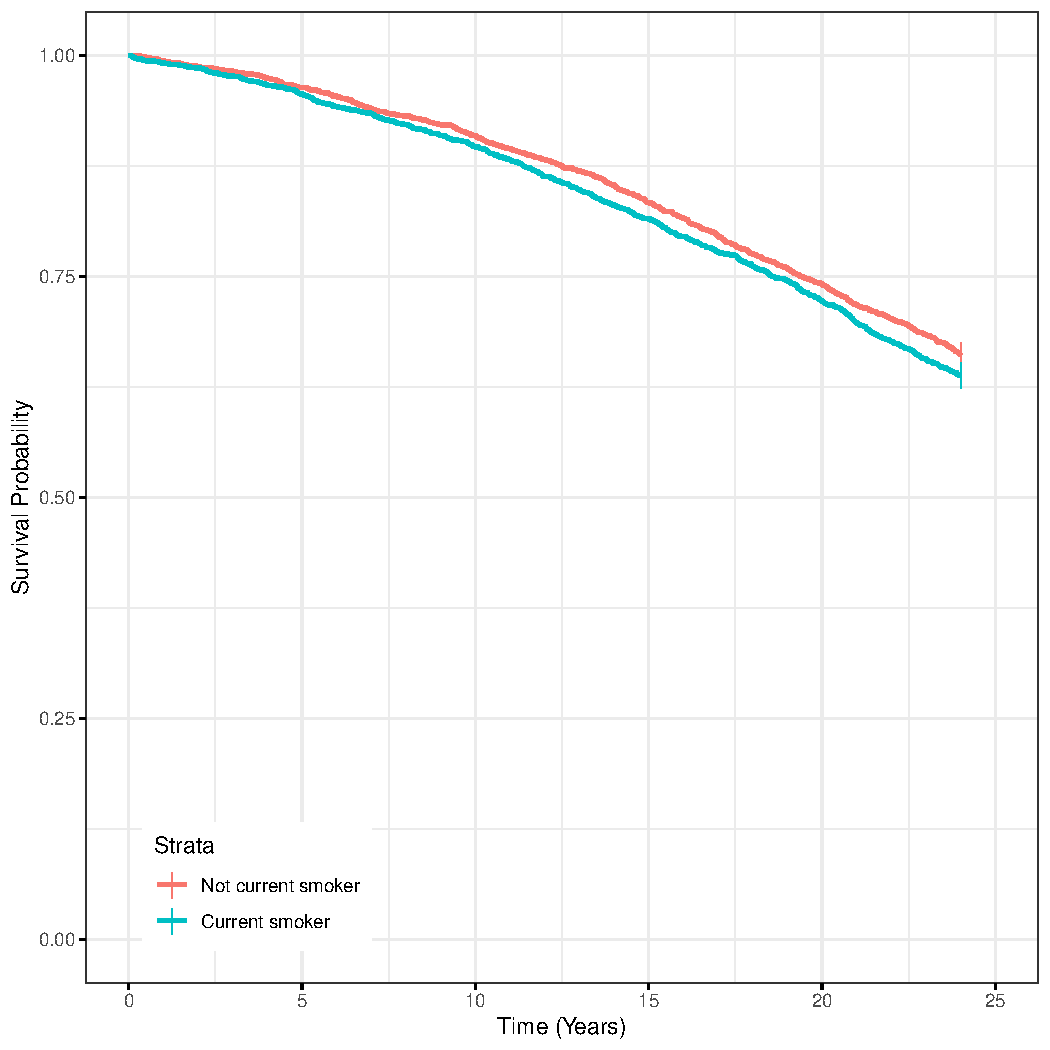
\includegraphics[width=\maxwidth]{figure/unnamed-chunk-15-1} 

\end{knitrout}

\pagebreak

\section*{Question 2}

\ifdraft

\textbf{Referring to the code from lecture}, are you able to calculate the overall median survival time in this case? If so, provide an estimate of this quantity, if not, describe why and provide an estimate of a percentile of survival time (of your choice). Interpret the quantity that you estimated. \textbf{(20 points)}

\vspace{2mm}



\fi

We cannot calculate the overall median survival time in this case because less than half of this sample had the event (death) by the end of the study.  (This dataset has no censored observations except for those right-censored at the end of the study, so the the number of participants observed to have died in this dataset equals the number who did actually die during the study period.)  In other words, over half of the observations are right-censored, and thus the true median survival time is somewhere in that majority of unobserved full survival times and unknown to us.  As over 25\% of the cohort did die over the course of the study, however, we can estimate the \textbf{25th percentile of survival time}, the first time point at which at least 25\% of the cohort had died and 75\% or less of the cohort remained alive, which was \textbf{19.09} years.  

\vspace{2mm}

(For another dataset containing censored observations throughout the study period instead of only at the end, a more accurate wording of the above might be "the first time point at which the probability of being dead in this cohort is estimated to be at least 25\%.  Both of those interpretations assume that all participants start counting follow-up time at the same time, whether in real or statistical time, which appears true for this dataset since all study entry times are 0.)

\vspace{2mm}

In other words, in this specific cohort with no censored observations until the end of the study and identical times of entry among all partiicpants, that last person who needed to die to bring the total percentage of the cohort dead to or above 25\% did so 19.09 years after the start of the study.

\vspace{2mm}

(The 25th percentile of survival time among current nonsmokers was 19.44 years, and the 25th percentile of survival time among current smokers was 18.61 years.  In other words, among members of the cohort who were nonsmokers at the beginning of the study, the first time at which at least 25\% of them had died was 19.44 years after the start of the study.  Similarly, the first time at which at least 25\% of the members of the cohort who were smokers at the beginning of the study had died was 18.61 years after the start of the study.)








\pagebreak

\section*{Question 3}

\ifdraft

Answer the following questions about the log-rank test: \textbf{(10 points total)}
  \begin{enumerate}
    \item Describe the specific null and alternative hypotheses that the log-rank test is considering here.
    \item What do you conclude from this test (use 5\% significance criteria)? List a limitation of the inference that you obtain from the log-rank test.
  \end{enumerate}

\fi

\subsection*{Sub-Question 1}

The null hypothesis for the log-rank test here is that the survival curve for the smokers is equivalent to that for the nonsmokers.  More specifically, the null hypothesis is that the probability of survival for a nonsmoker is the same as the probability of survival for a smoker at all times during the study period, or formally:

$$ H_0: S_1(t) = S_2(t) \: \forall(t) $$

where $S_k(t)$ is the survival probability for a member of group $k$ at time $t$.  (Here, $k=1$ designates the nonsmoking group and $k=2$ designates the smoking group.)

\vspace{2mm}

The alternative hypothesis is that the survival curve for at least one group is different than the others at some time during the study period, or, formally:

$$ \exists (t) \: S_1(t) \neq S_2(t) $$

\subsection*{Sub-Question 2}



The p-value of \textbf{0.09} indicates that we cannot reject the null hypothesis of no difference between the smoker and nonsmoker survival curves at the 5\% significance level.

\vspace{2mm}

One limitation of the log-rank test is that, although it allows for censoring, it requires that censoring to be non-informative, i.e., unrelated to survival probability.  (It also requires survival probabilities to be the same regardless of the entry date into the study, i.e., that survival probabilities are not affected by factors only present at specific dates when some participants were in the study and some were not.)  Another limitation is that, in the case of a significant result, the log-rank test does not identify the time or times at which the survival curves differ.  A third limitation of the log-rank test is its inability to distinguish, in the presence of more than two survival curves and a significant result, which curves are different without further testing.  A fourth limitation is that the log-rank test does not accommodate adjustment for covariates.

\pagebreak

\section*{Question 4}

\ifdraft

Answer the following questions about the Cox models estimated above: \textbf{(20 points total)}
  \begin{enumerate}
    \item Why do we use specialized methods for survival analysis (instead of linear or logistic regression, for example)? (Hint: See readings from Vittinghoff et al. 2012 text.)
    \item What are the advantages of the Cox model over other survival analysis methods? What is a potential disadvantage of the Cox model?
    \item What assumptions, if any, does the standard \textbf{Cox} proportional hazards model make?
    \item Compare the test of the smoking-mortality association between the log-rank test and the likelihood ratio test from the \ul{unadjusted} Cox proportional hazards model. What do you observe? Between these two analytic approaches, which one would you prefer, and why?
  \end{enumerate}

\fi

\subsection*{Sub-Question 1}
\textbf{Why do we use specialized methods for survival analysis (instead of linear or logistic regression, for example)?}

\vspace{2mm}

We use specialized methods for survival analysis in order to fully incorporate the information contained in varying follow-up times.  We cannot use linear regression (with survival time as the outcome) due to the right-censoring of the events of interest (e.g., disease incidence or death) frequently present in survival data, which often leaves many survival times unknown.  Worse, the missing survival times are censored informatively, meaning that whether a survival time is unknown is associated with the outcome of survival time, i.e., the longest times are the ones most likely to be missing.  Thus using linear regression on the known survival times would systematically underestimate them.  Adjusting for follow-up time can partially account for variations in follow-up time but imposes assumptions on the relationship between follow-up time and event risk (e.g., that follow-up time is associated with risk in some kind of linear manner).

\vspace{2mm}

We cannot use logistic regression, either, even though we are interested in the binary presence or absence of an event, because logistic regression ignores variation in follow-up times, which arises both from variation in participants' entry times into the study and from differences in survival times among participants.  Doing a simple logistic regression with event presence or absence at the end of the study as the outcome effectively ignores the information contained in the participant surivival times.  Moreover, if systematic differences exist in entry times between the groups of interest (for example, exposed participants generally entered the study later than unexposed participants), logistic regression could produce particularly biased results.  Pooled logistic regression, which looks at binary event outcomes at several times over the course of the study instead of only at the end, can help account for variations in follow-up times, but is more appropriate when events are discovered at regularly spaced intervals at which outcomes can be evaluated (e.g., study visits conducted at the same intervals for all participants) and still fails to incorporate the specific information garnered from having exact event times, producing less accurate estimates of event risk than survival analysis methods that can fully accommodate exact event times.

\subsection*{Sub-Question 2}
\textbf{What are the advantages of the Cox model over other survival analysis methods? What is a potential disadvantage of the Cox model?}

\vspace{2mm}

Advantages:
The Cox model does not require us to specify the distribution of the failure times $T$, also known as the baseline hazard.  Thus the Cox model is more robust than parametric proportional hazards models because bias cannot arise from misspecification of the distribution of failure times.

Disadvantage:
One potential disadvantage of the Cox model is the decreased precision (and increased variance) in the Cox model compared to fully parametric survival models that either specify the distribution of failure times accurately or are relatively robust to misspecifications.

\vspace{2mm}

\subsection*{Sub-Question 3}
\textbf{What assumptions, if any, does the standard \textit{Cox} proportional hazards model make?}

\vspace{2mm}

The standard Cox proportional hazards model assumes

\begin{itemize}
  \item That the covariates have multiplicative associations with the hazard (as they reside in the parametric portion of the model, in an exponent relative to the hazard), as opposed to additive or other associations;
  \item That the hazard ratios are constant over time (the \textit{proportional hazards assumption}), i.e., that the hazard in one group is a constant multiple of the hazard of any other group throughout time;
  \item That survival times are independent among study participants; 
  \item That measurements and times are accurate in the dataset; and
  \item That any censoring is uninformative, i.e., not associated with survival time.
  
\end{itemize}

\vspace{2mm}

\subsection*{Sub-Question 4}
\textbf{Compare the test of the smoking-mortality association between the log-rank test and the likelihood ratio test from the \ul{unadjusted} Cox proportional hazards model. What do you observe? Between these two analytic approaches, which one would you prefer, and why?}

\vspace{2mm}



Both the log-rank test and the likelihood ratio test from the unadjusted Cox proportional hazards model give nearly identical results, i.e., a chi-square statistic of 2.91 on one degree of freedom ($p = 0.088$).  Thus neither rejects the null hypothesis that no systematic difference in survival times exists between current smokers and nonsmokers at the 5\% significance level.  Were I not allowed to adjust for any other covariates, like here, I would prefer the log-rank test, as it is fully nonparametric and does not presume any prior relationship between the Kaplan-Meier survival curves on which it is based and is thus more robust to a wider variety of distributions of survival times among groups.  The Cox proportional hazards model, in contrast, assumes that hazard ratios (derived from relationships among survival curves) remain constant over time between any two groups.  Were I allowed to adjust for covariates, however, I would ultimately use the likelihood ratio test from the Cox proportional hazards model or some variation of it, as the Cox model can accommodate a wider variety of covariates and thus will ultimately produce more informed and accurate estimates of the relationship between a categorical exposure and survival time outcomes.

\vspace{2mm}

\pagebreak

\section*{Question 5}

\ifdraft

Write the equation for the log-hazard function for the \textit{adjusted} model you estimated. \textbf{Clearly define all functions, terms (covariates), and parameters in the model. (20 points)}

\fi

Equation:

$$ \log(h(t|\mathbf{x}, \boldsymbol{\beta})) =  \log[h_0(t)] + \beta_1\mathbb{I}(x_1 = 1) + \beta_2 x_2 + \beta_3\mathbb{I}(x_3 = 1) + \beta_4\mathbb{I}(x_4 = 2) + \beta_5\mathbb{I}(x_4 = 3) + \beta_6\mathbb{I}(x_4 = 4) $$

\vspace{2mm}
Definitions:

\begin{itemize}

  \item $ \log(h(t|\mathbf{x}, \boldsymbol{\beta})) $ is the natural logarithm of the instantaneous rate (hazard) of death at time $t$ for a participant who has survived up to that time $t$, given the covariates in $ \mathbf{x} $ and coefficients in $\boldsymbol{\beta}$;
  \item $\log(h_0(t))$ is the baseline instantaneous rate (hazard) of death at time $t$ for a participant who was not a current smoker, was zero years old, was male, had 0-11 years of education at the first examination, and survived up to time $t$;
  \item $\mathbf{x}$ is a vector of covariates containing
    \begin{itemize}
      \item $x_1$, an indicator variable for smoking corresponding to the dataset variable `cursmoke`, with $x_1 = 1$ indicating that the participant was a current smoker at the first examination and $x_1 = 0$ indicating that the participant was not;
      \item $x_2$, a continuous variable for age of the participant at the first examination in years;
      \item $x_3$, an indicator variable corresponding to the recoded variable `female` derived from the dataset variable `sex`, with $x_3 = 1$ indicating a female participant (originally `sex = 2`) and $x_3 = 0$ indicating a male participant (originally `sex = 1`);
      \item $x_4$, a four-category categorical variable corresponding to the dataset variable `educ`, where
        \begin{itemize}
          \item $x_4 = 1$ corresponds to the dataset variable `educ = 1`, indicating that the participant had 0-11 years of education (in this equation, this condition is the reference condition and subsumed in the baseline hazard term $\log[h_0(t)]$ tercept term $x_0 = 1$);
          \item $x_4 = 2$ corresponds to the dataset variable value `educ = 2`, indicating that the participant had a high school diploma or GED;
          \item $x_4 = 3$ corresponds to the dataset variable value `educ = 3`, indicating that the participant had some college or vocational school;
          \item $x_4 = 4$ corresponds to the dataset variable value `educ = 4`, indicating that the participant had a college degree or more;
      \end{itemize}
    \end{itemize}
  \item $\mathbb{I}()$ is the formula for an indicator variable, which equals 1 if the equation inside the parentheses is true and 0 if it is not (used to create indicator variables for each non-reference level of the categorical variables in $\mathbf{x}$);  
  \item $\boldsymbol{\beta}$ is a vector of coefficients including
    \begin{itemize}
      \item $\beta_1$ is the log hazard ratio comparing the hazard of death for a participant who was a current smoker at the first examination to the hazard of death for a participant who was not, holding the values of all other variables constant;
      \item $\beta_2$ is the log hazard ratio for a one-year increase in age, holding the values of all other variables constant,
      \item $\beta_3$ is the log hazard ratio comparing the hazard of death for a participant who was a female (in the numerator) to the hazard of death for a participant who was male (in the denominator) at the first examination, holding the values of all other variables constant;
      \item $\beta_4$ is the log hazard ratio comparing the hazard of death for a participant who had a high school diploma or GED (in the numerator) to the hazard of death for a participant who had 0-11 years of education (in the denominator) at the first examination, holding the values of all other variables constant;
      \item $\beta_5$ is the log hazard ratio comparing the hazard of death for a participant who had some college or vocational school (in the numerator) to the hazard of death for a participant who had 0-11 years of education (in the denominator) at the first examination, holding the values of all other variables constant;
      \item $\beta_6$ is the log hazard ratio comparing the hazard of death for a participant who had some college or vocational school (in the numerator) to the hazard of death for a participant who had a college degree or more (in the denominator) at the first examination, holding the values of all other variables constant.
    \end{itemize}
  \end{itemize}
      
\pagebreak

\section*{Question 6}

\ifdraft

Complete the following table. How would you interpret the parameter estimate that compares smokers to non-smokers in the \textbf{adjusted model}? What measure of association common in epidemiologic research does this correspond to? \textbf{(10 points)}

\fi







% latex table generated in R 3.6.1 by xtable 1.8-4 package
% Mon Nov 25 01:56:58 2019
\begin{table}[H]
\centering
\parbox{10cm}{\caption{Crude and adjusted hazard ratio (HR) estimates of the association between baseline smoking status and mortality. Framingham Cohort Study. 1948-1972, Framingham, MA.}} 
\begin{tabular}{lrrll}
  \hline
Smoker & Events & Follow-Up Time (years) & Crude HR (95\% CI) & Adjusted HR (95\% CI) \\ 
  \hline
No & 762 & 46675.20 & 1. (reference) & 1. (reference) \\ 
  Yes & 788 & 44440.38 & 1.091 (0.987—1.205) & 1.404 (1.262—1.562) \\ 
   \hline
\end{tabular}
\end{table}


The hazard of death during the study for a participant who was a current smoker at the start of the study was 1.404 times (95\% confidence interval: 1.262, 1.562) that of a participant who was not a current smoker at the start of the study after adjusting for age, sex, and level of education.  Hazard ratios, in general, correspond to incidence rate ratios.  (See the following reference for a discussion of why hazard ratios do not always approximate relative risks well: \textit{Sutradhar R and Austin PC. Relative rates not relative risks: addressing a widespread misinterpretation of hazard ratios. Annals of Epidemiology. 2018;28(1):54-57. doi:10.1016/j.annepidem.2017.10.014.})  That said, in the absence of competing events, rate ratios can approximate risk ratios.

\pagebreak

\section*{Question 7}

\ifdraft

Based on the model that included covariate-by-time interactions, is there evidence for a violation of the proportional hazards assumption in any of the variables? Indicate how you arrived at your conclusion. \ul{In 1-2 sentences} describe in general how you would account for any violations in the proportional hazards assumption (ignoring whether or not there were significant differences here). \textbf{(10 points)}

\fi

The sex variable appears to violate the proportional hazards assumption.  To evaluate violations of the proportional hazards assumption in the variables, I reran the adjusted model, adding interactions with time for all the covariates:

\begin{equation*}
\begin{split} 
\log(h(t|\mathbf{x}, \boldsymbol{\beta})) = \log[h_0(t)] + \beta_1\mathbb{I}(x_1 = 1) + \beta_2 x_2 + \beta_3\mathbb{I}(x_3 = 1) + \beta_4\mathbb{I}(x_4 = 2) + \beta_5\mathbb{I}(x_4 = 3) + \beta_6\mathbb{I}(x_4 = 4) \; + \\ \beta_7\mathbb{I}(x_1 = 1)\times t + \beta_8x_2\times t + \beta_9\mathbb{I}(x_3 = 1)\times t + \beta_{10}\mathbb{I}(x_4 = 2)\times t + \beta_{11}\mathbb{I}(x_4 = 3)\times t + \beta_{12}\mathbb{I}(x_4 = 4)\times t 
\end{split} 
\end{equation*}

All functions, covariates, and parameters have the same defnitions as in question 5, with the addition of the coefficients $\beta_7, \beta_8, \ldots, \beta_12$ to model possible interactions with time.  I then produced the table below, which shows a significant interaction at the 5\% significance level ($p = 0.026$) for the interaction between sex and time.  I then conducted a global likelihood ratio test comparing the log likelihood of the adjusted model with the time interaction to the same model without the time interaction, obtaining a significant chi-square value of 4.148 with one degree of freedom ($p = 0.042$), indicating that the interaction improves the model accuracy.

\vspace{2mm}

To account for a violation of the proportional hazards assumption: If the violation were in a confounder (e.g., in sex here), I would either include the time interaction(s) with the confounder in the model to account for its effects on the exposure-outcome association, or, if I could categorize the confounder easily and did not care about evaluating its association with the outcome, I would estimate a model stratified by the levels of that confounder to allow for a different baseline hazard function in each stratum.  If the violation were in the exposure of interest (e.g., in current smoking here), I would include all the time interactions in the model and report time-specific instead of overall effects.




% latex table generated in R 3.6.1 by xtable 1.8-4 package
% Mon Nov 25 01:56:58 2019
\begin{table}[H]
\centering
\parbox{11cm}{\caption{Estimates of associations between baseline smoking status and mortality including adjustment for potential interactions with time. Framingham Cohort Study. 1948-1972, Framingham, MA.}} 
\begin{tabular}{lrrrrr}
  \hline
Covariate & Beta & e\verb|^|Beta & Standard Error & z & p \\ 
  \hline
Current Smoker & 0.44 & 1.55 & 0.13 & 3.34 & 0.00 \\ 
  Age & 0.09 & 1.09 & 0.01 & 10.90 & 0.00 \\ 
  Female Sex & -0.29 & 0.75 & 0.13 & -2.24 & 0.02 \\ 
  Education: High School & 0.00 & 1.00 & 0.15 & 0.02 & 0.99 \\ 
  Education: Some College & -0.17 & 0.84 & 0.19 & -0.89 & 0.37 \\ 
  Education: College Degree & -0.26 & 0.77 & 0.22 & -1.16 & 0.25 \\ 
  Current Smoker by Time & -0.01 & 0.99 & 0.01 & -0.81 & 0.42 \\ 
  Age by Time Interaction & 0.00 & 1.00 & 0.00 & 1.10 & 0.27 \\ 
  Female by Time Interaction & -0.02 & 0.98 & 0.01 & -2.22 & 0.03 \\ 
  Education: High School by Time & -0.00 & 1.00 & 0.01 & -0.30 & 0.76 \\ 
  Education: Some College by Time & 0.00 & 1.00 & 0.01 & 0.02 & 0.99 \\ 
  Education: College Degree by Time & -0.00 & 1.00 & 0.01 & -0.34 & 0.73 \\ 
   \hline
\end{tabular}
\end{table}



\end{document}
